\documentclass{article}
\usepackage[letterpaper, total={7in, 8in}]{geometry}
\usepackage[utf8]{inputenc}
%\usepackage[english]{babel}
\usepackage[]{amsthm} %lets us use \begin{proof}
\usepackage[]{amsmath}
\usepackage[]{amssymb} %gives us the character \varnothing
\usepackage{mathrsfs}
\usepackage{graphicx}
\usepackage{adjustbox}
\usepackage{titlesec}
\usepackage[numbered,framed]{matlab-prettifier}
\usepackage{listings}
\usepackage[t1,OT1]{fontenc}
\usepackage{filecontents}
\usepackage{float}
\usepackage{physics}
\usepackage{csvsimple}
\usepackage{booktabs}
\usepackage{longtable}
\usepackage{algorithmicx}
\usepackage{mathtools}
\usepackage{breqn}
\usepackage{framed,color}
\usepackage{amsmath,mleftright}
\usepackage{xparse}
\usepackage{titling}
\usepackage{tabularx}
\usepackage{subcaption}

\usepackage{siunitx}
\usepackage{hyperref}

\setlength{\droptitle}{-10em}   % This is your set screw

\NewDocumentCommand{\evalat}{sO{\big}mm}{%
	\IfBooleanTF{#1}
	{\mleft. #3 \mright|_{#4}}
	{#3#2|_{#4}}%
}


\DeclareMathOperator{\atantwo}{atan2}

\titleformat{\section}{\normalfont\Large\bfseries}{Section \thesection.}{1em}{}
\titleformat{\subsection}{\normalfont\bfseries}{\alph{subsection})}{1em}{}
%\definecolor{shadecolor}{gray}{0.9}

\title{Smart Products Final Project Report}
\author{Yuan Gao and Tyler Morrison}
\date\today

%\lstset{
%	style              = Matlab-editor,
%	basicstyle         = \mlttfamily,
%	escapechar         = ",
%	mlshowsectionrules = true,
%	literate = {-}{-}1, % <hyphens will not show up unless you add this
%}

\lstset{
	language=C++,
	basicstyle=\ttfamily,
	keywordstyle=\color{blue}\ttfamily,
	stringstyle=\color{red}\ttfamily,
	commentstyle=\color{green}\ttfamily,
	morecomment=[l][\color{magenta}]{\#},
	numbers=left,
	stepnumber=1,
	frame=single
}

\renewcommand{\lstlistingname}{Program}% Listing -> Algorithm

\begin{document}
\maketitle

All of our code can be found in a remote Git repository at \url{https://github.com/tymo77/smart-products}. A video of the robot picking can be watched here: \url{https://www.youtube.com/watch?v=LKYOw6bc5pM}. This method was very reliable during testing. I'd estimate our reliability was greater than 90\% however, Tyler made a simple mistake during the demo that caused it to be slightly off. A video of the working elevator code can be seen here: \url{https://www.youtube.com/watch?v=miOiRZVIvwA}. These two sets of code are not dependent. They can be compiled and run separately so, in order to simplify development, they are two different executables, written and compiled in the \href{https://github.com/tymo77/smart-products/tree/master/labs/project}{\texttt{project}} and \href{https://github.com/tymo77/smart-products/tree/master/labs/project_motors}{\texttt{project\_motors}} directories.


\section{Communication logic}
To realize a stable and reliable communication between Pi and camera, we utilized the logic shown below

\begin{figure}[H]
	\centering
	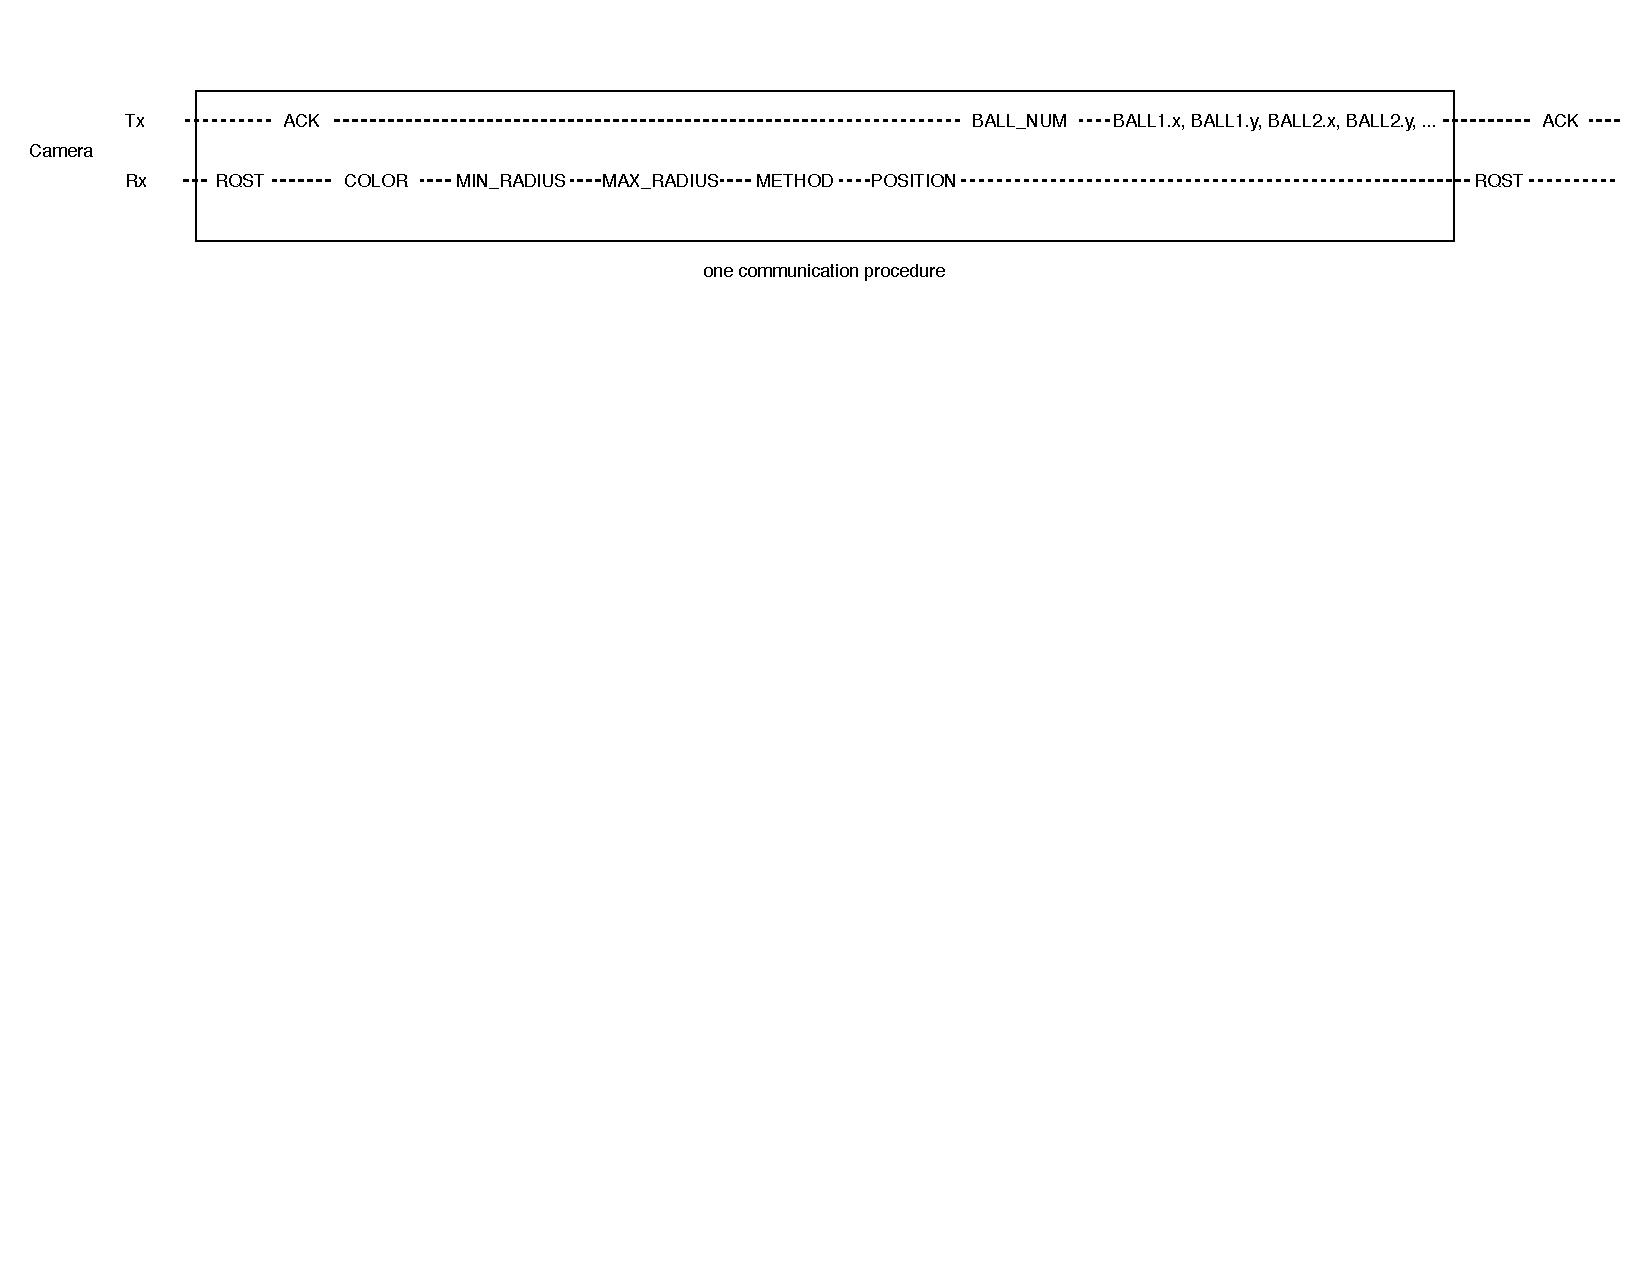
\includegraphics[keepaspectratio,width=.95\linewidth]{communication.pdf}
	\caption{Example of our communication protocol.}
\end{figure}

\begin{figure}[H]
	\centering
	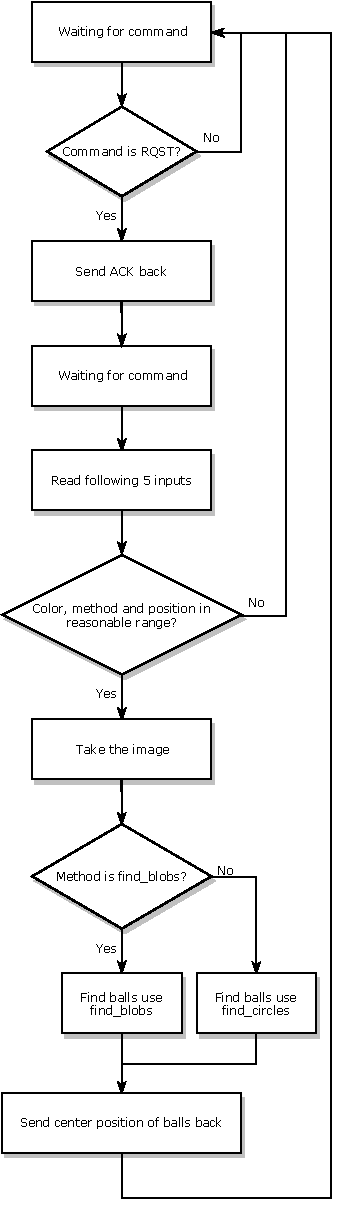
\includegraphics[keepaspectratio,height=\textheight]{camera_pseudo.pdf}
	\caption{Camera software.}
\end{figure}%

\noindent Here we define two handshake codes: request and acknowledgment, two color codes for red and green, two method codes respectively represent \texttt{find\_circles} and \texttt{find\_blobs} function and three position codes that stand for three positions of the dobot. Minimum and maximum radius are used to limit the size of circle detected by \texttt{find\_circles} function and increase the precision. These nine defined codes range from 1 to 9 and are different with each other to avoid misreading. After receiving and verifying the validness of all input parameters, the camera will detect all the balls in desired color at region of interest determined by Dobot position and return the number of balls and then the list of balls’ center position.


\section{Color selection}
We have two methods to detect the ball and the ways to determine the color are different.
For \texttt{find\_circles} function:
Because we can’t set the preferred RGB value range in the function, after getting the list of circles, we derive the average RGB value in the detected ball area and determine whether a ball is red or green based on the R and G value.
For \texttt{find\_blobs} function:
In \texttt{find\_blobs} function, LAB value can be used to find blobs in certain color. We obtained the LAB value tuple for red and green by capturing the ball region in the image. Find\_blob function give us rectangle regions in desired color and the center of the blob is the center of the ball. 

\section{Overall Algorithm}
First we input coordinates for the ramp drop off locations and the home location to scan the scene from. Then we scan the scene, pick a target and move toward it. We stop above it, scan and move to a set height above it. We repeat this process several times to hone in then move in to pick it. We then lift it and carry it to the appropriate ramp and release. After all of the desired colors have been collected and placed, we lift the ramp gates to load the elevator and then lift the elevators to the appropriate height and release the appropriate ramp each time.

\begin{figure}[H]
		\centering
		\includegraphics[keepaspectratio,height=\textheight]{SP_project_flowchart.pdf}
		\caption{Algorithm.}
\end{figure}

\section{Methods of Note}

\subsection{Calibration between Camera and Robot}
\begin{figure}[H]
	\centering
	\begin{subfigure}{.49\textwidth}
		\centering
		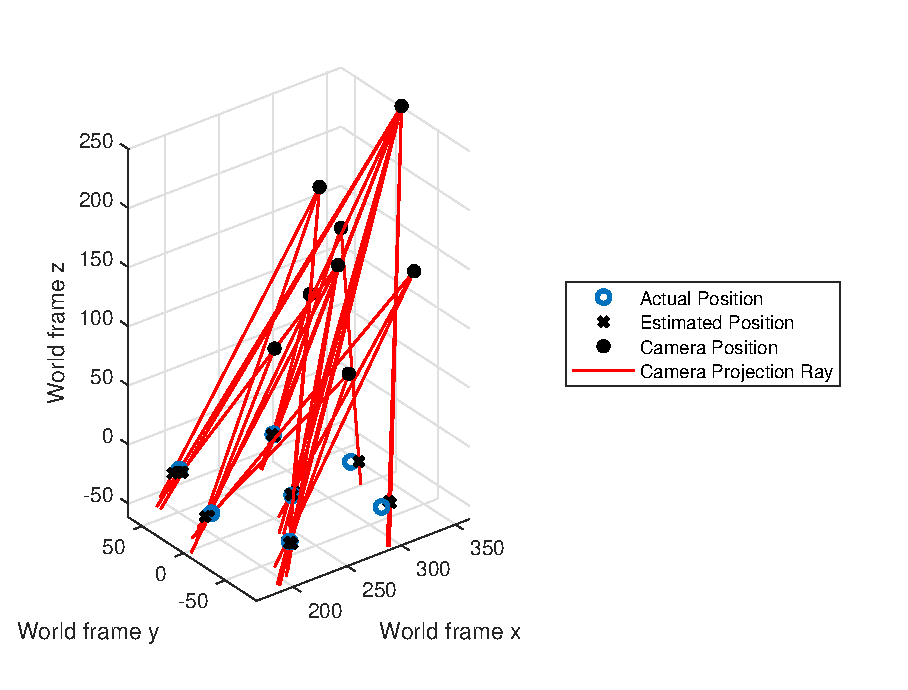
\includegraphics[keepaspectratio,width=\linewidth]{calibration1.eps}
	\end{subfigure}%
	\begin{subfigure}{.49\textwidth}
		\centering
		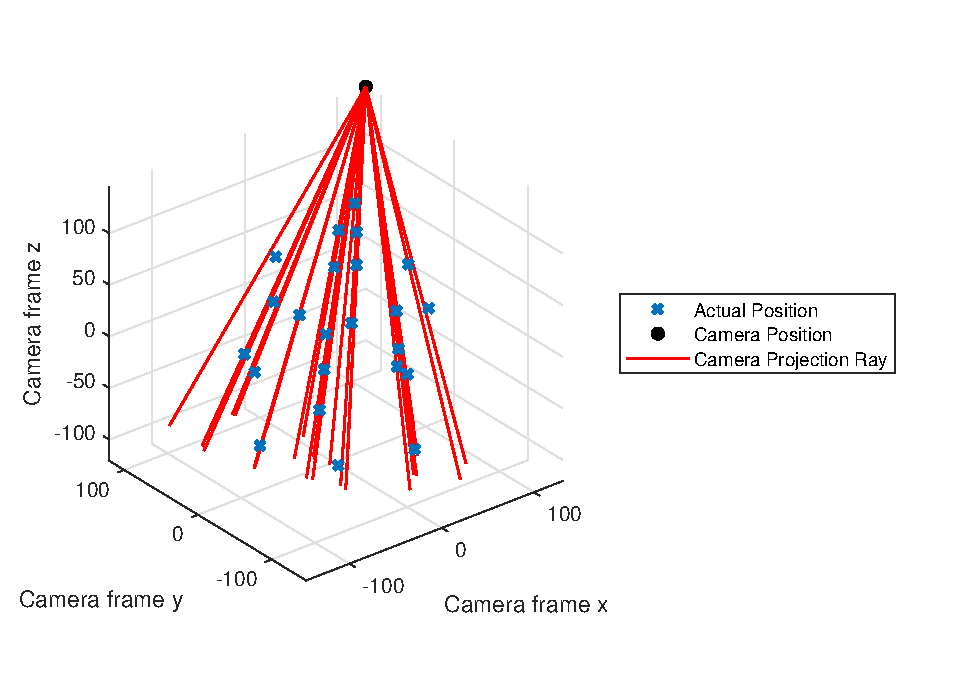
\includegraphics[keepaspectratio,width=\linewidth]{calibration2.eps}
	\end{subfigure}
	\caption{Graphics of the calibration process to translate from xy coordinates in the image to xyz coordinates in the frame of the last link.}
\end{figure}

In order to be able to get the position of a ball in the world xyz frame from its place in the camera image we make use of the following ideas: 1) Each pixel on the camera corresponds to a ray of possible locations in 3D space in the camera xyz frame (that was set somewhere in space relative to the camera during calibration). 2) The balls all sit on a plane of (basically) constant z in the world xyz frame. 3) There is a constant 3D rigid body transformation from the camera frame to the frame of the third link of the robot because that is where the camera is fixed.

Points 1) and 2) are implemented by solving equations of line intersection with a plane and getting the equation of the line. Dylan has described methods for this before, but we had already developed our own code for this. 

Point 3) is implemented by calibration. Several balls are placed in the workspace with positions recorded by placing the end effector gently on their center top. Then, several images are taken of the scene from different positions and the position of the robot for that image as well as the image positions of the centers of the balls are recorded for each detected ball and paired with their known coordinates in the world frame. The image centers of the positions of the balls are used to create a set of lines in the camera frame. The known positions of the balls and the robot coordinates for each image are used to construct a set of points in link coordinates that correspond to each line in the camera frame. The correct rigid body transformation between these two is found by minimization of the distance between each point in camera space (after being transformed by the rigid body transformation we are solving for) and its corresponding projection line. The result is an accurate 3D rigid body transformation to convert camera image coordinates to camera xyz coordinates to link xyz coordinates to world frame xyz coordinates -- all without needing to measure the position of the camera relative to the third link. 

\subsection{Using Make and command line arguments to speed testing and integration}
Throughout the lab, in order to decrease compile times during each iteration of testing, we used a handcrafted Makefile to do efficient compilation. Make will only compile files affected by recent changes. Compiling each library and linking them afterward allows minor changes to be made without waiting for the entire codebase to recompile.

We also made use of command line arguments. By passing different flags to our main routine in \texttt{project} various simple tasks can be accomplished without commenting out lines in the mainfile and recompiling. We include options such as:

\begin{tabular}{ll}
	\texttt{-L} & Load previous saved home and ramp positions.\\
	\texttt{--get-pos} & Print out current robot pose coordinates. \\
	\texttt{--go-to} & Move robot to xyz coordinates. \\
	\texttt{--suction-off} & Turn off suction. \\
	\texttt{--suction-on} & Turn on suction. \\
\end{tabular}

\end{document}